\subsection{The material, $\beta$-Ga$_2$O$_3$}

The primitive unit cell of $\beta$-Ga$_2$O$_3$ is base-centered monoclinic with the unit cell parameters listed in Table \ref{tab:unitcell_parameters}, which is in the space group C2/m. The structure has three inequivalent oxygen sites and two inequivalent gallium sites. The unit cell is shown in Figure \ref{fig:unit_cell}. The oxygen sites are named O(I), (OII) and O(III). O(I) and O(II) are threefold coordinated, while O(III) is fourfold coordinated (see Figure \ref{fig:oxygen_sites}). The gallium sites are called Ga(I) and Ga(II). Ga(I) and Ga(II) are tetrahedrally and octahedrally coordinated, respectively \cite{dft_ga2o3}. Figure \ref{fig:gallium_sites} shows the different sites in the super cell. Figure \ref{fig:distances} shows which gallium atoms the 'different' oxygens are bonded to and the length of the bonds. The lengths are from the relaxed super cell.

\begin{table}[H]\caption{This is the unit cell parameters for the $\beta$-Ga$_2$O$_3$ primitive unit cell.}\label{tab:unitcell_parameters}
\begin{tabular}{ll}                          
a = 12.23000 Å &       $\alpha$ = 90.0000\degree \\
b =  3.04000 Å &      $\beta$ =103.7000 \degree \\
c =  5.80000 Å &     $\gamma$ = 90.0000 \degree \\
V = 209.5042 $\text{Å}^3$& \\
\end{tabular}
\end{table}

\begin{figure}[H]
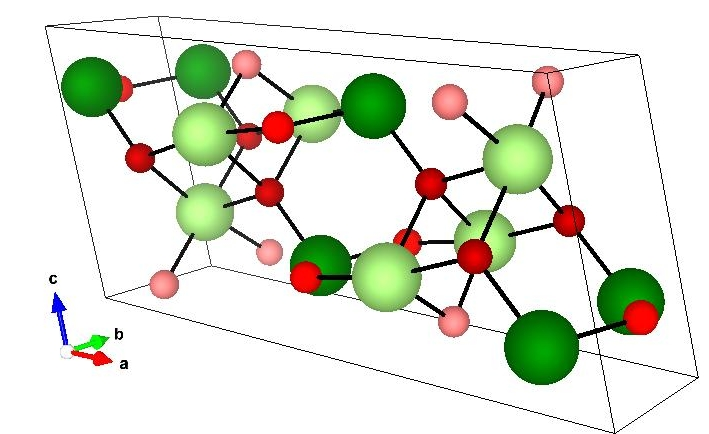
\includegraphics[width=\linewidth]{../fig/unitcell}\caption{This figure shows the primitive unit cell of $\beta$-Ga$_2$O$_3$.}\label{fig:unit_cell}
\end{figure}

\begin{figure}[H]
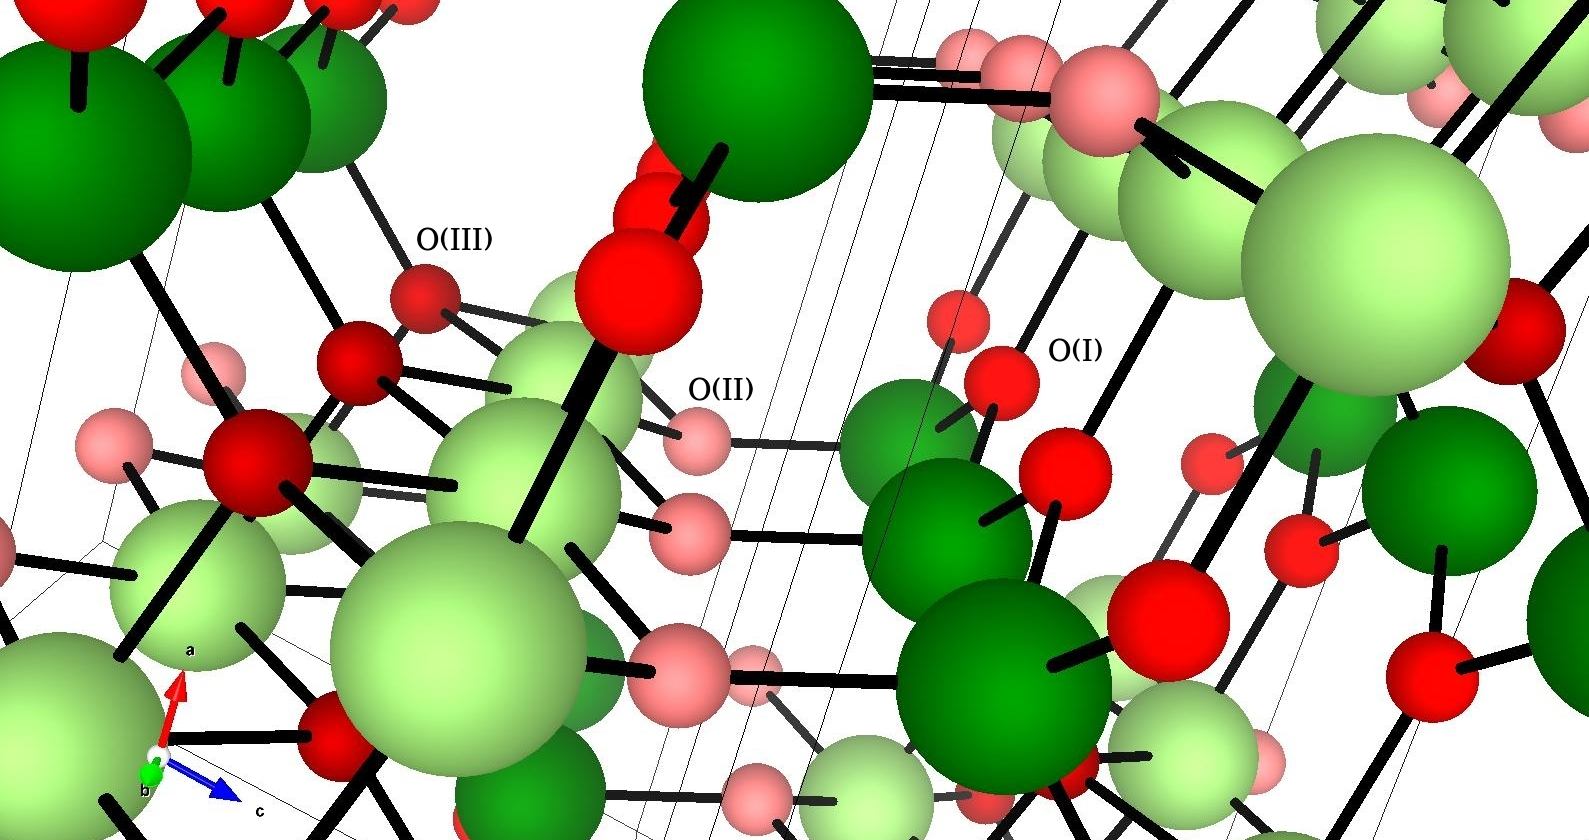
\includegraphics[width=\linewidth]{../fig/Ga2O3-different-sites-names}\caption{This figure shows the inequivalent oxygens in the unit cell. There are three different oxygen sites, they are color coded and named.}\label{fig:oxygen_sites}
\end{figure}

\begin{figure}[H]
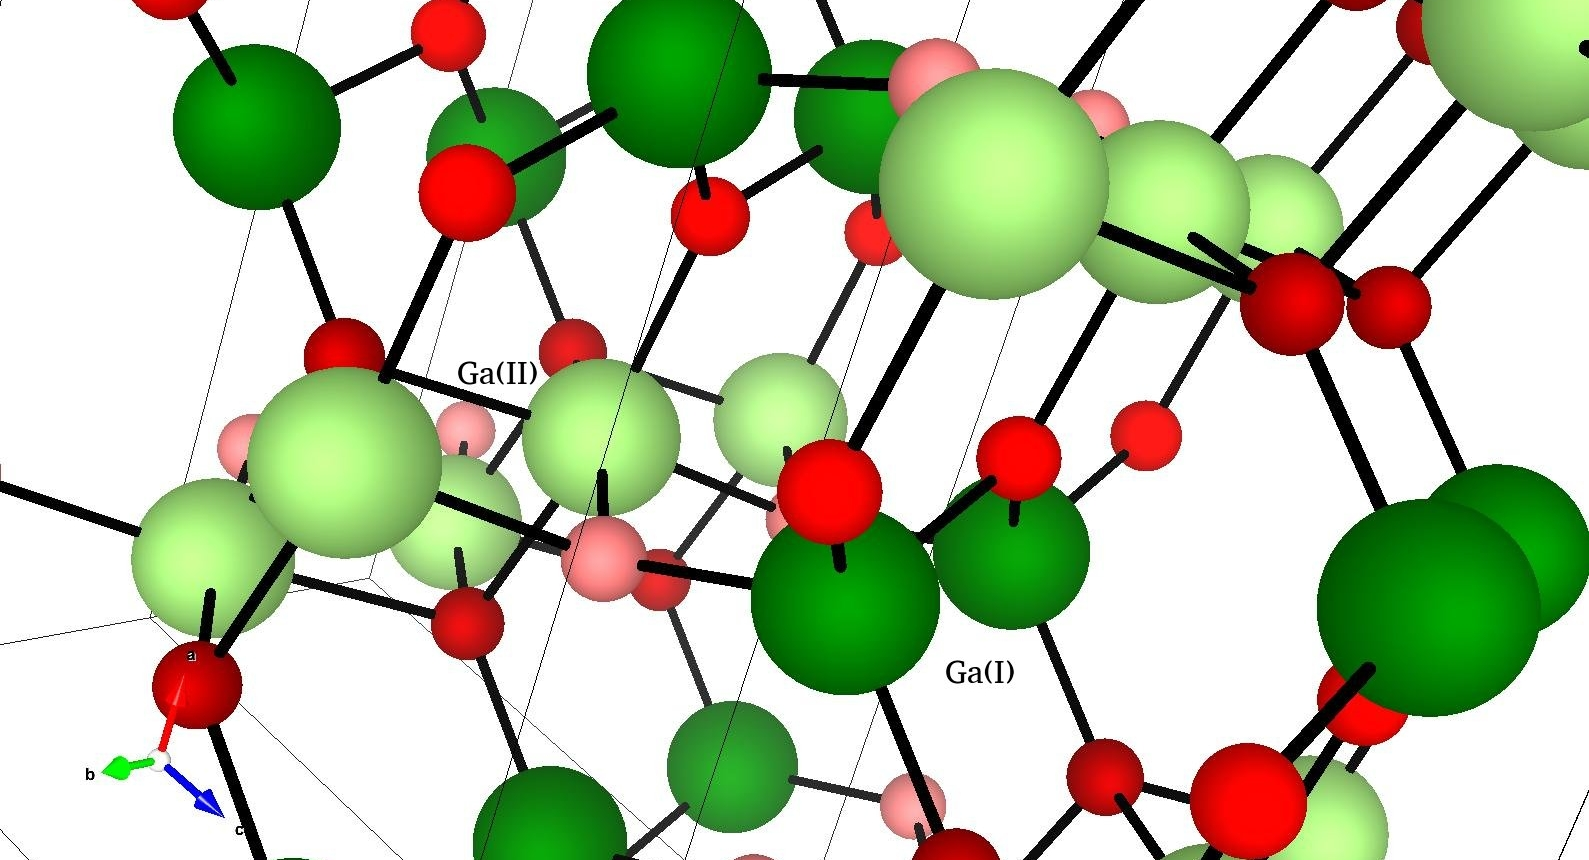
\includegraphics[width=\linewidth]{../fig/Ga2O3-Ga-sites}\caption{This figure shows the inequivalent gallium sites in the unit cell.}\label{fig:gallium_sites}
\end{figure}

\begin{figure}[H]
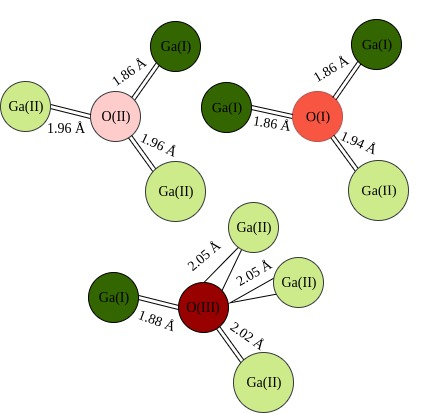
\includegraphics[width=\linewidth]{../fig/distances}\caption{This figure shows the distances at the different oxygen sites in the relaxed super cell. We assume that the distances are similar for all equivalent sites in the supercell, because these are the distances for a three specific ones.}\label{fig:distances}
\end{figure}

\subsection{DFT Convergence}

The first thing one does when doing DFT calculations are convergence tests. This is important because it gives data one can use to consider how accurate the resulting properties will be, compared to how costly the calculations are. The more accurate results, the higher cost in CPU time. A convergence test will also show if numerical noise gives a limit to the accuracy of the result.

The convergence of a relative change in energy, relative change in force and relative change in pressure versus energy cut-off and k-point density is checked. The energy cut-off is a value that represent the limit of the infinite sum over G-vectors (see Equation \ref{eq:energy_cutoff}). We cannot sum an infinite sum, so we have to choose a limit that is sufficient for the accuracy we want to achieve. Because it is a sum over G-vectors, the energy cut-off has to be big for localized states. Oxygen has localized states and that indicates that this material need a high energy cut-off for good accuracy. 

\begin{equation}\label{eq:energy_cutoff}
E_{cut-off} = \sum \frac{1}{G}
\end{equation}

The k-point density is related to the k-point mesh of the numerical integral over k-vectors. Because it involves k-vectors it is related to more unlocalized states and metallic materials might need high k-point density because of their electrons delocalized states. $\beta$-Ga$_2$O$_3$ is a semiconductor though and might not need a high k-point density.

The properties are chosen to be the relative change because it is easier to converge and the total energy from DFT calculations are not that interesting physically because it is not a physical number. It is simply a numerical one. The relative change in energy is interesting though because then one can compare different situation. The comparison is physically interesting because it is independent of the real total value. 

After choosing a convergence criteria, the accuracy one wants or settles at, the energy cut-off and the k-point density can be used to relax the structure. When relaxing the structure, the program minimizes the maximum force felt by the the atoms in the structure and, if one chooses to, minimizes the pressure. The energy cut-off and the k-point density is used for all the calculations; relaxation, the total energy and density of states calculations.

\subsection{DFT Formation Energy}

When comparing total energies from DFT calculations, it is important to compare the energy for the same amount of atoms. That means that if one compares the energy of a material with the energy of the material with a vacancy, as we will do in this project, one has to add the energy of the atom giving the vacancy in vacuum. In this case the vacancy is an oxygen vacancy and the energy of an oxygen molecule in vacuum also has to be calculated. This difference will give the formation energy of the oxygen vacancy.

The formation energy of the oxygen vacancy is actually also dependent on the temperature, pressure and the charge of the vacancy. The equation for calculating the formation energy is given in Equation \ref{eq:formation_energy_complicated} where $E_{vac}$ is the total bulk energy with the vacancy, $E_b$ is the total bulk energy without the vacancy, $P$ is the pressure, $\mu_O$ is the chemical potential of oxygen given by Equation \ref{eq:mu_O}. $E_{tot}^{O_2}$ is the total energy of the oxygen molecule in vacuum, $ \tilde{\mu}_{O_2}$ is the difference from $T= 0$ K at the reference pressure, $P_0$, and can be found in tables, $kT\log(\frac{P}{P_0})$ represents the difference in pressure, $P$, form the reference pressure and the last term represent the impact of a charged vacancy where $q$ is the charge, $\epsilon_f$ is the Fermi level (or energy \ref. ) and $\epsilon_{VBM}$ is the maximum of the valence band.

\begin{equation}\label{eq:formation_energy_complicated}
E_f = (E_{vac} + \sum_i N_i \mu_i) - E_b + q(\epsilon_F + \epsilon_{VBM})
\end{equation}

\begin{equation}\label{eq:mu_O}
\mu_O = \frac{1}{2}\mu_{O_2} = \frac{1}{2}\left( E_{tot}^{O_2}+ \tilde{\mu}_{O_2} + kT\log(\frac{P}{P_0}) \right)
\end{equation}

In this project the setup is simple, the temperature is 0 K and the sample is assumed to be in oxygen rich conditions and in vacuum (how can it be in both o-rich and vacuum \ref. ). This makes the chemical potential of O$_2$, $\mu_{O_2} = E_{tot}^{O_2}$. The oxygen vacancy is also made to be neutral, not charged. A changed oxygen vacancy is a donor in the semiconductor, but if is is neutral the Fermi level is not changed and the term $q(\epsilon_F + \epsilon_{VBM})  = 0$. That is why the formation energy is simply given by Equation \ref{eq:formation_energy} where $\mu_O$ is simply given by Equation \ref{eq:mu_O_simple}.

\begin{equation}\label{eq:formation_energy}
E_f = (E_{vac} + \mu_O) - E_b
\end{equation}

\begin{equation}\label{eq:mu_O_simple}
\mu_O = \frac{1}{2} E_{tot}^{O_2}
\end{equation}